Dette afsnit bygger på \cite{sandsynlighedsBog} og \cite[]{grimsandsynlighedsBog}.
\section{Markovs ulighed}
\begin{theorem}
Hvis $X$ er en tilfældig variable med en begrænset middelværdi, så gælder
\begin{align*}
    P(|X|\geq a) \leq \frac{E[|X|]}{a} \text{ for alle } a > 0
\end{align*}
\end{theorem}
\begin{proof}
Lad $A=\{|X|\geq a\}$, så fremstilles indikator funktionen af $A$ $|X|\geq aI_a$. Så tages den forventede værdi på begge sider, hvorefter man kan flytte $a$ uden for.
\begin{align*}
E[|X|]\geq E[aI_a] = a E[I_a]
\end{align*} 
Til sidst divideres der med $a$ på begge sider. Eftersom den forventede værdi af indikartor funktionen er $P(A)$, så indsættes dette og giver det ænskede resultat.
\begin{align*}
    \frac{E[|X|]}{a} \geq P(A)
\end{align*} 
\end{proof}
Det er værd at bemærke at hvis $a<0$ så skal relationen vendes om.

\section{Chebyshews ulighed}
Chebyshews ulighed siger noget om hvad sansyndligheden er for at en tilfældig værdi ligger inden for $c$ gange standardafvigelser for middelværdien. Dette kan andvendes på enhver fordeling. 
\begin{theorem}
    Lad $X$ være en tilfældig variable med middelværdien $\mu$ og variansen $\sigma^2$. For alle konstanter $c>0$ gælder at 
    \begin{align*}
        P(|X-\mu|\geq c \sigma)\leq \frac{1}{c^2}
    \end{align*} 
\end{theorem}
\begin{proof}%fra wiki
    \begin{align*}
        P(|X-\mu|\geq c \sigma)=P((X-\mu)^2\geq k^2\sigma^2)
    \end{align*}
Fra \textbf{Markovs ulighed} vides det at, når $Y$ er en tilfædig variable og $a$ er positiv, gælder at $P(|Y|>a)\leq E(|Y|)/a$. Dette anvendes her
\begin{align*}
    P((X-\mu)^2\geq k^2\sigma^2) \leq \frac{E[(X-\mu)^2]}{c^2\sigma^2}
\end{align*}
Da $E[(X-\mu)]$ er definitionen af $\sigma$, så indsættes dette og beviset afsluttes.
\begin{align*}
    \frac{E[(X-\mu)^2]}{c^2\sigma^2} = \frac{\sigma^2}{c^2\sigma^2} = \frac{1}{c^2}
\end{align*}
\end{proof}
\section{Law of large numbers}
Law of large numbers går kort sagt ud på at ved en test med stor antal forsøg vil den emperiske middelværdien, nærme sig den teoretiske middelværdi, jo flere forsøg der bliver foretaget.
\begin{thm}%theorem 4.1
    Lad $X_1, X_2, \dots$ være en sekvens af iid. med tilfældige variabler, med middelværdien $\mu$, of lad $\Bar{X}$ være den emperiske middelværdi. For hver $\epsilon>0$ gælder at
    \begin{align*}
        P(|\Bar{X}-\mu|>\epsilon) \rightarrow 0 \text{ når } n \rightarrow \infty
    \end{align*}
\end{thm}
\begin{proof}
    Antag at $X_k$ har en afgrænset varians, dvs $\sigma^2<\infty$. Anvend \textbf{CHEBYSHEVS} ulighed på $\Bar{X}$, og lad $c=\epsilon \sqrt{x}/\sigma$. Eftersom $E[\Bar{X}]=\mu$ og $Var[\Bar{X}]=\sigma^2/n$, dermed giver det
    \begin{align*}
        P(|\Bar{X}-\mu| > \epsilon) \leq \frac{\sigma}{n\epsilon^2} \rightarrow 0 \text{ når } \rightarrow \infty
    \end{align*}
\end{proof}
Dermed vises det at når $n$ går imod uendelig, så går $\frac{\sigma^2}{n\epsilon^2}$ imod $0$, og at sandsynligeheden for at differensen mellem den teoretiske og den emperiske middelværdi er større end $\epsilon$, som er lig med eller mindre end $\frac{\sigma^2}{n\epsilon^2}$, som dermed også går imod 0, når $n$ går imod uendelig.

\section{Simulering af diskrete variable} 
Vi vil i følgende afsnit antage at vi har en stokastisk variabel $U \sim \unif[0,1]$\footnote{Vi vil ikke gå mere i dybten vedrørende simulering af kontinuerte uniforme variable}, som vi vil benytte til at simulere diskrete variable, givet deres pmf.
\begin{thm} \label{thm:simuleringAfDiskreteVaraible}
    Lad $p$ være en pmf over det diskrete udfaldsrum $\{x_1, x_2, \ldots\}$, lad $F_0 = 0$ og
    \begin{equation*}
        F_n = \sum^n_{k = 1} p(x_k), \text{ for } n \in \N.
    \end{equation*}
    Antag at $U \sim \unif[0, 1]$, og definer $X = x_n$ hvis $F_{n - 1} < U \leq F_n$, så har $X$ pmf $p$.
\end{thm}

\begin{proof}
    Da $U \sim \unif[0, 1]$ samt $X = x_n$ hvis og kun hvis $F_{n - 1} < U \leq F_n$ er
    \begin{equation*}
        P(X = x_n) = P(F_{n - 1} < U \leq F_n) = F_n - F_{n - 1} = p(x_n)
    \end{equation*}
    fordi $P(F_{n - 1} < U \leq F_n) = P\left(U \leq (F_n - F_{n - 1})\right)$.
\end{proof}

\begin{rem}
Hvis $p$ har tilhørende cdf $F$, så gælder det at $F_n = F(x_n)$ for $n \geq 1$. Følgende algoritme følger af sætning \ref{thm:simuleringAfDiskreteVaraible}, og gør det muligt at simulere diskrete fordelinger, givet den ønskede pmf $p$ og en uniform stokastisk variabel $U$ på intervallet $[0, 1]$.
\end{rem}

\begin{algorithm} 
\caption{Simulering af diskrete fordelinger}\label{alg:discreteSimulation} 
\begin{algorithmic}[1] 
\Procedure{Discrete Distrubution} {$p: \{x_1, x_2, \ldots\} \rightarrow [0, 1]$, $U \sim \unif[0, 1]$}
 %$p$ er pmf'en for variablen som ønskes simuleret.
    \State $S := 0$
    \For{$k \in N$}
        \State $S' := S + p(x_k)$ 
        \If{$S < U \leq S'$} \Return $x_k$
        \EndIf
        \State $S := S'$
    \EndFor
\EndProcedure
\end{algorithmic}
\end{algorithm} 



\begin{exmp} \label{exmp:simuleringAfDiskreteVariable}
    Det ønskes at simulere $X \sim \Poi(1)$. Så har $X$ pmf $p(k) = \dfrac{\e^{-1}}{k!}$ for $k \in \N_0$.
    
    Algoritme \ref{alg:discreteSimulation} implementeres i appendix \ref{app:kodeTilSimuleringAfDiskreteVariable}. Her simuleres $n$ stokastiske variable som følger Poisson fordelingen og måler samtidig frekvensen $F_k$ af hvert udfald i udfaldsrummet $\N_0$.
    Per \textbf{LAW OF LARGE NUMBERS}, kan vi approximere $p(k)$ som $\frac{F_k}{n}$ for $k = 0, 1, \ldots$, det benytter vi herefter til at lave følgende plot. 
    \begin{figure}[H]
        \centering
        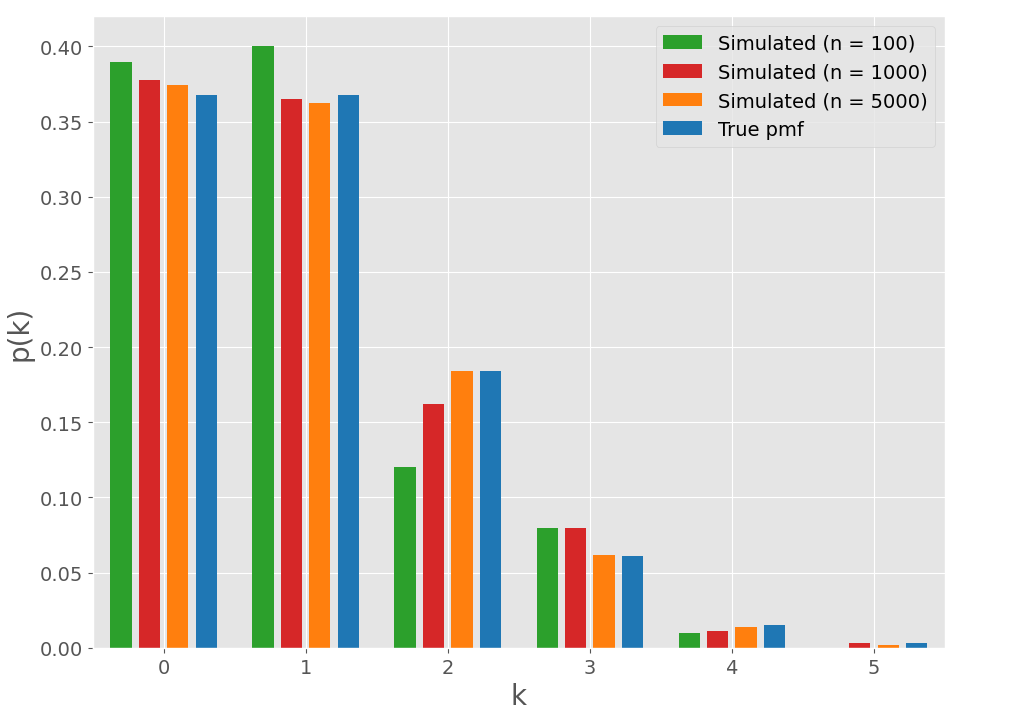
\includegraphics[scale=0.5]{fig/img/poisson.png} 
        \caption{Den simulerede relative frekvens af $k = 0, 1, \ldots, 5$ og den rigtige pmf.}
        \label{fig:simuleringAfPoisson}
    \end{figure}
    Det kan umiddelbart ses at den simulerede relative frekvens af $k$ går imod $p(k)$, når $n$ vokser.
\end{exmp}

